\begin{itemize}
    \item The idea is to combine the results of multiple classifiers for the same problem.
    \item \textbf{Bias} is the systematic deviation of its predicted decision boundary from the true decision boundary
    \item \textbf{Variance} is the deviation among the learned decision boundaries over different training sets.
    \item \textbf{Unstable classifier} is when small perturbations in the training set will result in large changes in the prediction. They have High variance and are subject to Overfitting.
    \item \textbf{Less complex classifiers} underfit the data, and usually have low variance, high bias.
    \item So we use Base Classifiers: trained on different subsets of data and produce Combined Classifier. With the Objective is to reduce bias and variance where we model complex classifiers using many simple ones.
    
\begin{figure}[H]
\centerline{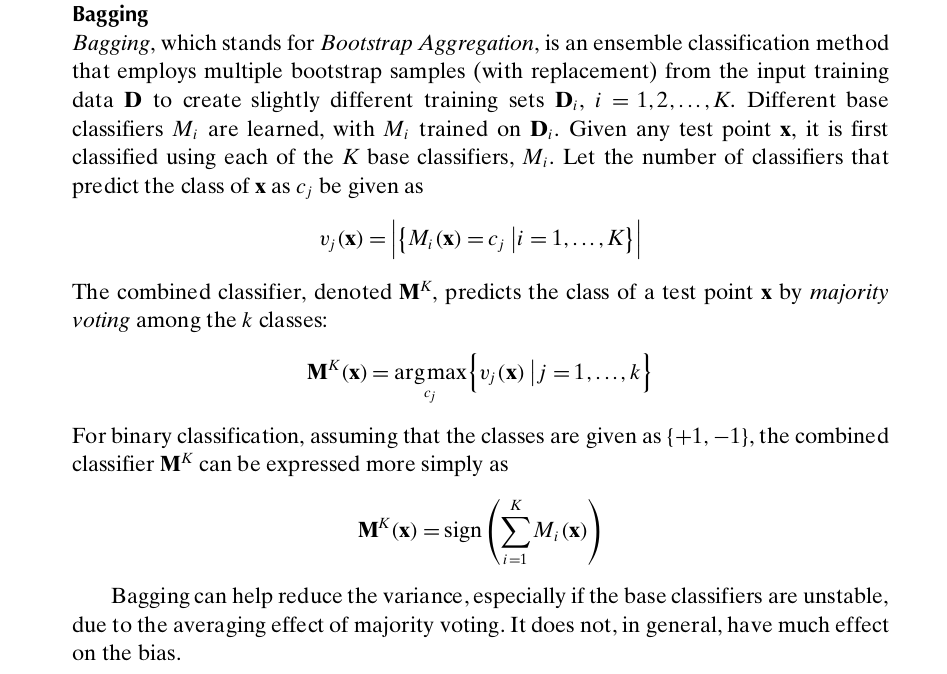
\includegraphics[width=1.2\textwidth]{Figures/bagging}}
\caption{\label{fig:figure}Bagging Method}
\end{figure}
\begin{figure}[H]
\centerline{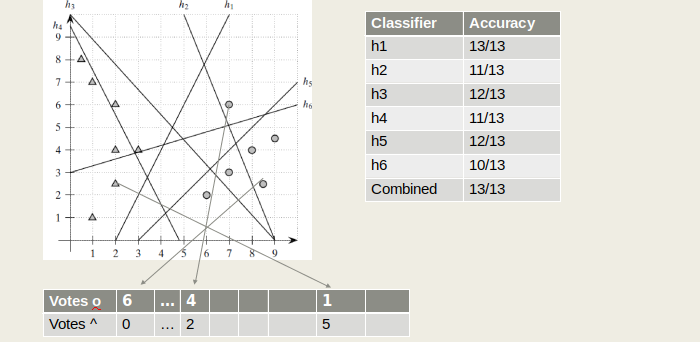
\includegraphics[width=\textwidth]{Figures/bagging2}}
\caption{\label{fig:figure}Example on Bagging Method}
\end{figure}


\begin{figure}[H]
    \centering
    \begin{minipage}{0.9\textwidth}
        \centering
        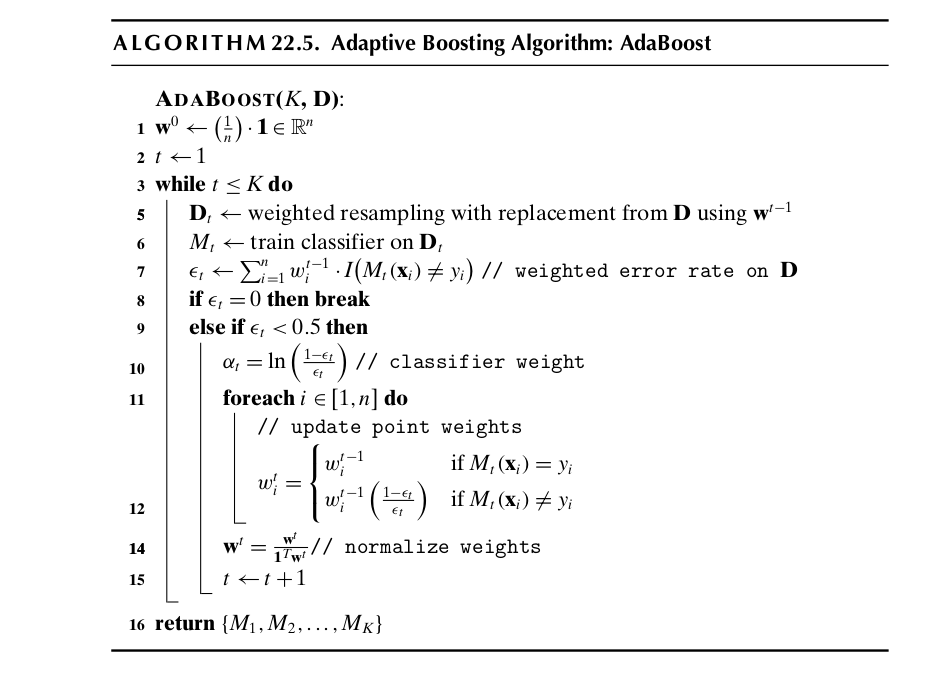
\includegraphics[width=\textwidth]{Figures/adaboost.png} % first figure itself
        \caption{Procedure}
    \end{minipage}\hfill
    \begin{minipage}{0.4\textwidth}
        \centering
        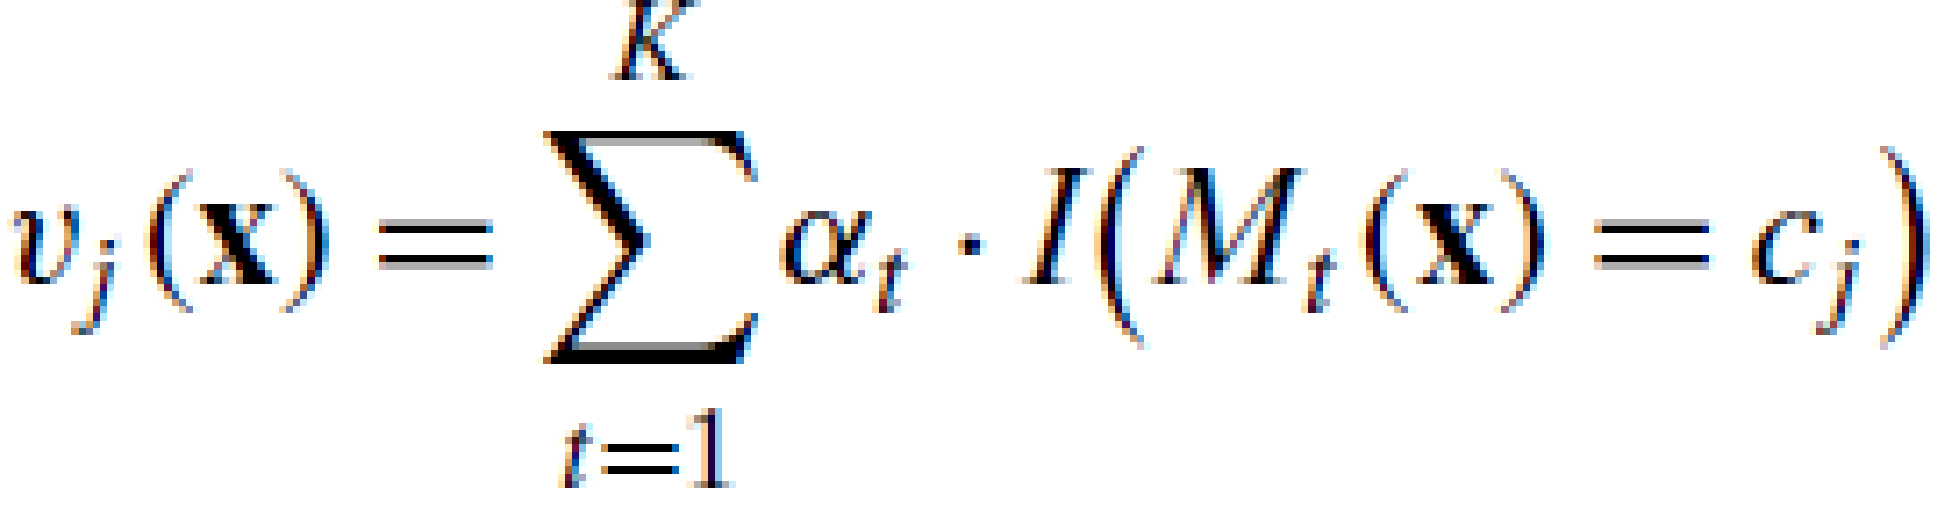
\includegraphics[width=\textwidth]{Figures/adaboost3.png} % second figure itself
    \end{minipage}
        \begin{minipage}{0.4\textwidth}
        \centering
        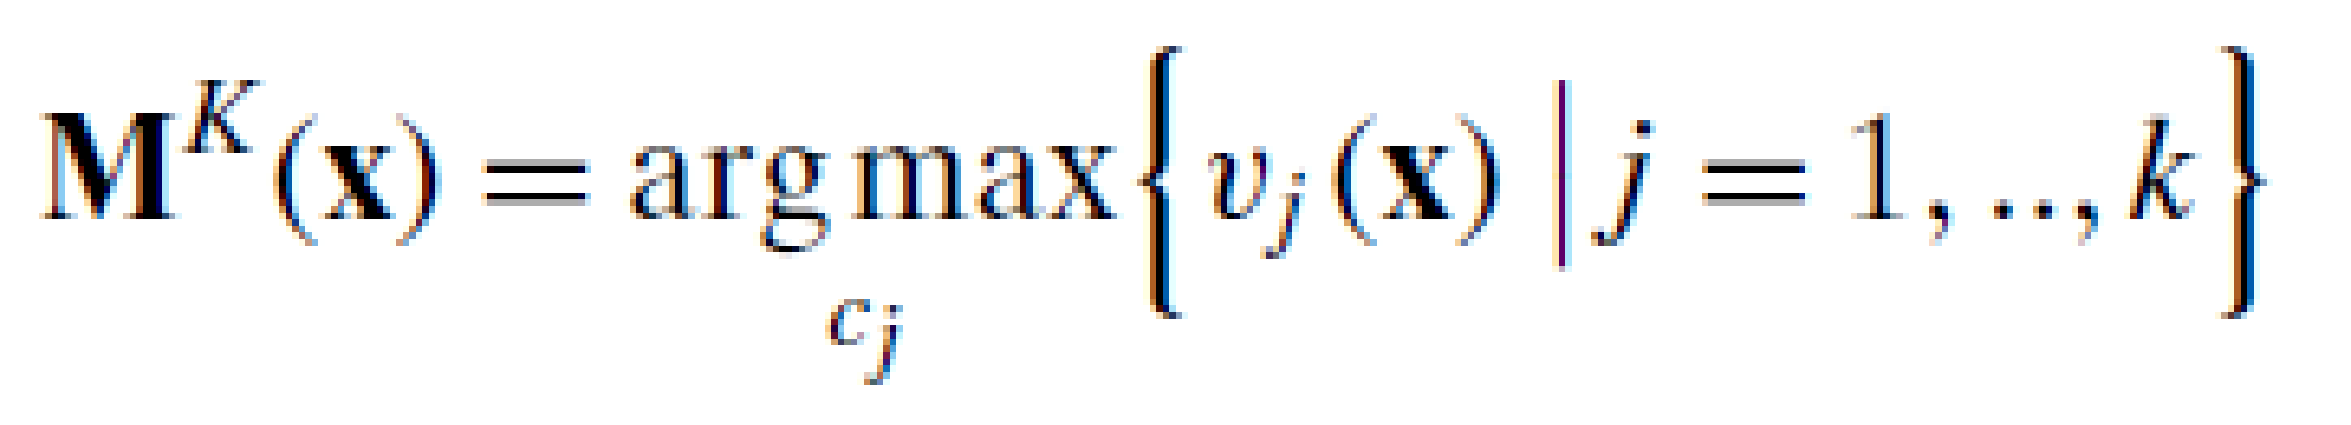
\includegraphics[width=\textwidth]{Figures/adaboost4.png} % second figure itself
    \end{minipage}
\end{figure}
\begin{figure}[H]
\centerline{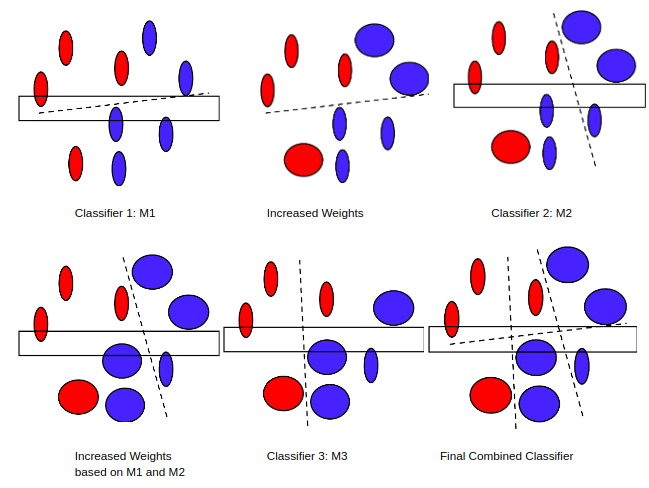
\includegraphics[width=1.2\textwidth]{Figures/adaboost2}}
\caption{\label{fig:figure}Example on Adaboost Method}
\end{figure}
    \item AdaBoost Notes
    \begin{itemize}
        \item Multiclass support? Yes. It can work for multi-class classification	
        \item Causes Reduction of variance due to averaging and Reduction of bias due to selecting harder examples
        \item Bagging is a special case of adaboost with Equal prob. of samples and Equal prob. of classifiers weights. It Reduces variance due to averaging.
        \item Supports non-linearity.
        \item May overfit the data.
    \end{itemize}




\end{itemize}